\documentclass[10pt,a4paper,oneside]{beamer}
\usepackage[utf8]{inputenc}
\usepackage{amsmath}
\usepackage{amsfonts}
\usepackage{amssymb}
\usepackage{graphicx}
\usepackage{breqn}
\usepackage{tikz} % system block diagram
\usepackage{textcomp}
\usetikzlibrary{shapes,arrows} % system block diagram
\usepackage{booktabs}
\usepackage[framed,numbered,autolinebreaks,useliterate]{mcode} % matlab code block
\author{Yangang Cao}
\newcommand{\degree}{^\circ}
\tikzset{
	delay/.style    = {draw, thick, rectangle, minimum height = 3em,
		minimum width = 3em},
	sum/.style      = {draw, circle, node distance = 2cm}, 
	prod/.style     = {draw, circle, node distance = 2cm},
	input/.style    = {coordinate}, % Input
	output/.style  = {coordinate} % Output
}
% Defining string as labels of certain blocks.
\newcommand{\product}{$\displaystyle \times$}
\newcommand{\delay}{\large$z^{-1}$}
%\documentclass[aspectratio=169]{beamer}
\usepackage[english]{babel}

% 加导航条
%\useoutertheme[width=3\baselineskip,right]{sidebar}
% 目录标数字
\setbeamertemplate{section in toc}[sections numbered] 
% 无序列表用实心点
\setbeamertemplate{itemize item}{$\bullet$}
% 设置每页标题格式
\setbeamertemplate{frametitle}
{\vspace{-0.5cm}
	\insertframetitle
	\vspace{-0.5cm}}
% 去掉下面没用的导航条
\setbeamertemplate{navigation symbols}{}
% 设置页脚格式
\makeatother
\setbeamertemplate{footline}
{
	\leavevmode%
	\hbox{%
		\begin{beamercolorbox}[wd=.4\paperwidth,ht=2.25ex,dp=1ex,center]{author in head/foot}%
			\usebeamerfont{author in head/foot}\insertshortauthor
		\end{beamercolorbox}
		
		\begin{beamercolorbox}[wd=.6\paperwidth,ht=2.25ex,dp=1ex,center]{title in head/foot}%
			\usebeamerfont{title in head/foot}\insertshorttitle\hspace*{13em}
			\insertframenumber{} / \inserttotalframenumber\hspace*{0ex}
	\end{beamercolorbox}}
	
	\vskip0pt%
}
\makeatletter


% 定义颜色
%\definecolor{alizarin}{rgb}{0.82, 0.1, 0.26} % 红色
%\definecolor{DarkFern}{HTML}{407428} % 绿色
%\colorlet{main}{DarkFern!100!white} % 第一种设置方法
%\colorlet{main}{red!70!black} % 第二种设置方法
\definecolor{bistre}{rgb}{0.24, 0.17, 0.12} % 黑色
\definecolor{mygrey}{rgb}{0.52, 0.52, 0.51} % 灰色
\colorlet{main}{green!50!black}
\colorlet{text}{bistre!100!white}

% 不同元素指定不同颜色,fg是本身颜色,bg是背景颜色,!num!改变数值提供渐变色
\setbeamercolor{title}{fg=text}
\setbeamercolor{frametitle}{fg=main}
\setbeamercolor{section in toc}{fg=text}
\setbeamercolor{normal text}{fg=text}
\setbeamercolor{block title}{fg=main,bg=mygrey!14!white}
\setbeamercolor{block body}{fg=black,bg=mygrey!10!white}
\setbeamercolor{qed symbol}{fg=main} % 证明结束后的框颜色
\setbeamercolor{math text}{fg=black}
% 设置页脚对应位置颜色
\setbeamercolor{author in head/foot}{fg=black, bg=mygrey!5!white}
\setbeamercolor{title in head/foot}{fg=black, bg=mygrey!5!white}
\setbeamercolor{structure}{fg=main, bg=mygrey!10!white} % 设置sidebar颜色

% 左右页间距的排版
\def\swidth{1cm}
\setbeamersize{sidebar width right=\swidth}
\setbeamersize{sidebar width left=\swidth}
\setbeamerfont{title in sidebar}{size=\scriptsize}
\setbeamerfont{section in sidebar}{size=\tiny}


%-------------------正文-------------------------%

\author{Yangang Cao}
\title{First-Order Low/High-Frequency Shelving Filter Design}
\date{February 18, 2019}

\begin{document}
	
	\frame[plain]{\titlepage}
	



\begin{frame}

 Definition of shelving filter:
\vspace{0.3cm}

Shelving filters boost or cut the low- or high-frequency bands with the parameters cut-off frequency $f_c$ and gain $G$, first-order low/high frequency shelving filters can be constructed based on a first-order allpass filter.

\end{frame}


\begin{frame}

The first-order low/high frequency shelving filters can be constructed based on a first-order allpass, yielding the transfer function
\[
H(z) = 1 + \frac{H_0}{2}[1 \pm A(z)]\quad(LF/HF+/-)
\]
with the first-order allpass
\[
A(z) = \frac{z^{-1} + c_{B/C}}{1 + c_{B/C}z^{-1}}.
\]
\end{frame}

\begin{frame}
Block diagram of first-order low/high-frequency shelving filter:
\begin{center}
	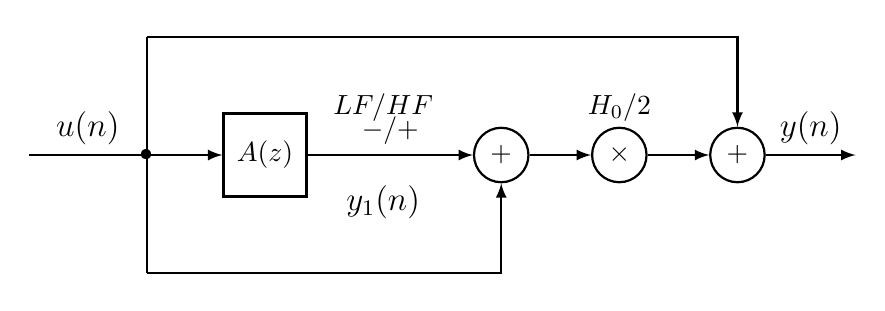
\begin{tikzpicture}[auto, thick, node distance=0.6cm, >=latex, scale = 0.75]
	\draw
	node at (2,0)[delay] (d1) {$A(z)$}
	node at (6,0)[sum] (s1) {$+$}
	node at (8,0)[prod](p1){$\times$} node[above of = p1]{$H_0/2$}
	node at (10,0)[sum](s2){$+$}
	node at (4,0)(n1){}
	node[above of = n1]{$LF/HF$} node[below of =n1]{\large$y_1(n)$}
	;
	
	\draw[-](-2,0) -- node {\large$u(n)$}(0,0);
	\draw[->](0,0) -- node {} (d1);
	\draw[->](d1) -- node {$-/+$} (s1);
	\draw[-](0,0) -- node {} (0,-2);
	\draw[->](0,-2) -| node {} (s1);
	\draw[->](s1) -- node {} (p1);
	\draw[->](p1) -- node {} (s2);
	\draw[->](s2) -- node {\large$y(n)$} (12,0);
	\draw[-](0,0) -- node {} (0,2);
	\draw[->](0,2) -| node {} (s2);
	
	\draw
	node at (0,0) {\textbullet};
	\end{tikzpicture}
\end{center}
\end{frame}

\begin{frame}
The difference equations of first-order low frequency shelving filter are
\[
x(n) = u(n) - c_{B/C}x(n-1)
\]
\[
y_1(n) = c_{B/C}x(n) + x(n-1)
\]
\[
y(n) = \frac{H_0}{2}[u(n) + y_1(n)] + u(n).
\]
and corresponding state and output equations are
\[
x(n) = -c_{B/C}x(n-1) + u(n)
\]
\[
y(n) = \frac{H_0}{2}(1-c^2)x(n-1) + [\frac{H_0}{2}(1+c)+1]u(n)
\]
\end{frame}
\begin{frame}[fragile]
Matlab code:
\begin{lstlisting}
function y = lowshelvingunit(audio, para)
% Applies a low-frequency shelving filter to the input signal.
% para(1) is the normalized cut-off frequency in (0,1), i.e. 2*fc/fs
% para(2) is the gain in dB
V0 = 10^(para(2)/20); H0 = V0 - 1;
if para(2) >= 0
    c = (tan(pi*para(1)/2)-1) / (tan(pi*para(1)/2)+1);     % boost
else
    c = (tan(pi*para(1)/2)-V0) / (tan(pi*para(1)/2)+V0);   % cut
end
x = 0;
x_1 = 0;
for n=1:length(audio)
    x_1 = -c * x + audio(n);
    y(n) = H0 / 2 * (1-c^2) * x + [H0 / 2 * (1+c) + 1] * audio(n);
    x = x_1;
end
\end{lstlisting}
\end{frame}

\begin{frame}
The difference equations of first-order high frequency shelving filter are
\[
x(n) = u(n) - c_{B/C}x(n-1)
\]
\[
y_1(n) = c_{B/C}x(n) + x(n-1)
\]
\[
y(n) = \frac{H_0}{2}[u(n) - y_1(n)] + u(n).
\]
and corresponding state and output equations are
\[
x(n) = -c_{B/C}x(n-1) + u(n)
\]
\[
y(n) = \frac{H_0}{2}(c^2-1)x(n-1) + [\frac{H_0}{2}(1-c)+1]u(n)
\]
\end{frame}
\begin{frame}[fragile]
Matlab code:
\begin{lstlisting}
function y = highshelvingunit(audio, para)
% Applies a high-frequency shelving filter to the input signal.
% para(1) is the normalized cut-off frequency in (0,1), i.e. 2*fc/fs
% para(2) is the gain in dB
V0 = 10^(para(2)/20); H0 = V0 - 1;
if para(2) >= 0
    c = (tan(pi*para(1)/2)-1) / (tan(pi*para(1)/2)+1);     % boost
else
    c = (tan(pi*para(1)/2)-V0) / (tan(pi*para(1)/2)+V0);   % cut
end
x = 0;
x_1 = 0;
for n=1:length(audio)
    x_1 = -c * x + audio(n);
    y(n) = H0/2 * (c^2-1) * x + (H0/2 * (1-c) + 1) * audio(n);
    x = x_1;
end
\end{lstlisting}
\end{frame}
\end{document}